%------------------------------------------------------
%
%   Mijenjati po potrebi, i to u vlastitom predavanju!
%
%   Za promjene u samom predlošku,
%   konzultirajte osobu zaduženu za održavanje.
%
%------------------------------------------------------

\documentclass[crop=false, class = scrartcl]{standalone}

\usepackage[utf8]{inputenc}
\usepackage[T1]{fontenc}
\usepackage[croatian]{babel}

 
\usepackage{csquotes} % za prave navodnike

\usepackage{subfiles} % da mogu različiti fileovi funkcionirat
\usepackage{amsmath, amssymb, amsthm} % hrpa matematičkih formula/znakova
\usepackage{enumitem} % formatiranje numeriranja

\usepackage{graphicx} % za slike
\graphicspath{ {./images/} }

\usepackage[dvipsnames]{xcolor} % za bojanje
%tikzpicture
\usepackage{tikz}
\usepackage{scalerel}
\usepackage{pict2e}
\usepackage{tkz-euclide}
\usetikzlibrary{calc}
% siunitx config
\RequirePackage{siunitx}
\sisetup{per-mode = symbol} % show m/s instead of ms^-1
\sisetup{output-decimal-marker = {,}}
\DeclareSIUnit\liter{\litre} % small L in litres
\DeclareSIUnit\euro{\geneuro}
\sisetup{output-decimal-marker = {,}}
\usetikzlibrary{patterns,arrows.meta}
\usetikzlibrary{shadows}
\usetikzlibrary{external}
\usetikzlibrary{intersections}
\usetikzlibrary{angles}

\usepackage{multirow} %
\usepackage{multicol} % za formatiranje naslova

\usepackage{fontawesome} % za ove unicode ikone

\usepackage[top=2cm,bottom=2cm,left=2cm,right=2cm]{geometry} % margine stranica

%\usepackage{biblatex}
%\addbibresource{literatura.bib}

\setlength{\parindent}{0cm} % da se odlomci ne uvlače
\pagenumbering{gobble} % za nenumeriranje
\frenchspacing

\definecolor{orange_mnm}{HTML}{F37021}
\definecolor{grey_mnm}{HTML}{666666}

%Formatiranje poglavlja i potpoglavlja
\renewcommand*{\sectionformat}{\LARGE{\color{orange_mnm!80!}\thesection.}\enskip}
\renewcommand*{\subsectionformat}{\large{\color{orange_mnm!80!}\thesubsection.}\enskip}
\renewcommand*{\subsubsectionformat}{\large{\color{orange_mnm!80!}\thesubsubsection.}\enskip}

%Bitno za formatiranje naslova!
\usepackage{array}
\newcolumntype{L}[1]{>{\raggedright\let\newline\\\arraybackslash\hspace{0pt}}m{#1}}
\newcolumntype{C}[1]{>{\centering\let\newline\\\arraybackslash\hspace{0pt}}m{#1}}
\newcolumntype{R}[1]{>{\raggedleft\let\newline\\\arraybackslash\hspace{0pt}}m{#1}}

% TEOREMSKA OKRUZENJA:
\usepackage[framemethod = tikz]{mdframed} % za namještanje theorem tip environmenata
\usetikzlibrary{shadows}
\usepackage{thmtools} % za lakše editanje theorem tip 

\makeatletter
\define@key{thmdef}{mdthm}[{}]{%
\thmt@trytwice{\def\thmt@theoremdefiner{\mdtheorem[#1]}}{}}
\makeatother

\mdfdefinestyle{thmstyle}{
linewidth = 1.5pt,
linecolor = orange_mnm!90!,
hidealllines = true,
leftline = true,
innerleftmargin = 3pt,
innerrightmargin = 3pt,
frametitleaboveskip = 5pt,
frametitlebelowskip = 5pt,
frametitlerule = false,
frametitlebackgroundcolor = orange!5,
frametitlefont = \sffamily\bfseries,
shadow = true,
shadowsize = 4pt,
shadowcolor = black!5!
}

\declaretheoremstyle[
  headfont=\normalfont\itshape,
  spacebelow = 2pt,
  spaceabove = 12pt
]{italic}
		
\mdfdefinestyle{defstyle}{
linewidth = 1.5pt,
linecolor = RoyalBlue!90!green!,
hidealllines = true,
leftline = true,
innerleftmargin = 3pt,
innerrightmargin = 3pt,
frametitleaboveskip = 5pt,
frametitlebelowskip = 5pt,
frametitlerule = false,
frametitlebackgroundcolor = RoyalBlue!5,
frametitlefont = \sffamily\bfseries,
shadow = true,
shadowsize = 4pt,
shadowcolor = black!5!
}

\mdfdefinestyle{lemstyle}{
linewidth = 1.5pt,
linecolor = ForestGreen!90!black!,
hidealllines = true,
leftline = true,
innerleftmargin = 3pt,
innerrightmargin = 3pt,
frametitleaboveskip = 5pt,
frametitlebelowskip = 5pt,
frametitlerule = false,
frametitlebackgroundcolor = ForestGreen!5,
frametitlefont = \sffamily\bfseries,
shadow = true,
shadowsize = 4pt,
shadowcolor = black!5!
}

\mdfdefinestyle{napstyle}{
linewidth = 1.5pt,
linecolor = Plum!90!black!,
hidealllines = true,
leftline = true,
innerleftmargin = 3pt,
innerrightmargin = 3pt,
frametitleaboveskip = 5pt,
frametitlebelowskip = 5pt,
frametitlerule = false,
frametitlebackgroundcolor = Orchid!10,
frametitlefont = \sffamily\bfseries,
shadow = true,
shadowsize = 4pt,
shadowcolor = black!5!
}

\mdfdefinestyle{oprstyle}{
linewidth = 1.5pt,
linecolor = WildStrawberry!90!black!,
hidealllines = true,
leftline = true,
innerleftmargin = 3pt,
innerrightmargin = 3pt,
frametitleaboveskip = 5pt,
frametitlebelowskip = 5pt,
frametitlerule = false,
frametitlebackgroundcolor = Salmon!10,
frametitlefont = \sffamily\bfseries,
shadow = true,
shadowsize = 4pt,
shadowcolor = black!5!
}

\declaretheoremstyle[
  headfont=\color{ForestGreen!80!black}\sffamily\bfseries,
  spacebelow = 2pt,
  spaceabove = 12pt
]{primjersty}

\declaretheoremstyle[
  headfont=\color{RawSienna!60!red!}\sffamily\bfseries,
  spacebelow = 6pt,
  spaceabove = 6pt
]{rjesenjesty}

%\declaretheorem[mdthm = {style = thmstyle}, name = {{\bfseries\sffamily\color{orange_mnm!30!orange!} \faInfoCircle} Teorem}, numberwithin = section]{teorem}
\declaretheorem[mdthm = {style = thmstyle}, name = {Teorem}, numberwithin = section]{teorem}
%\declaretheorem[mdthm = {style = thmstyle}, name = {{\bfseries\sffamily\color{orange_mnm!30!orange!} \faInfoCircle} Propozicija}, sibling = teorem]{propozicija}
\declaretheorem[mdthm = {style = thmstyle}, name = {Propozicija}, sibling = teorem]{propozicija}
\declaretheorem[mdthm = {style = thmstyle}, name = {Poučak}, sibling = teorem]{poucak}
%\declaretheorem[mdthm = {style = thmstyle}, name = {{\bfseries\sffamily\color{orange_mnm!30!orange!} \faInfoCircle} Korolar}, sibling = teorem]{korolar}
\declaretheorem[mdthm = {style = thmstyle}, name = {Korolar}, sibling = teorem]{korolar}
\declaretheorem[name = Dokaz, numbered = no, style = italic, qed = $\qedsymbol$]{dokaz}
%\declaretheorem[name = {\bfseries\sffamily {\color{RoyalBlue!30!blue!} \faInfoCircle} Definicija}, mdthm = {style = defstyle}, sibling = teorem]{definicija}
\declaretheorem[name = {Definicija}, mdthm = {style = defstyle}, sibling = teorem]{definicija}
%\declaretheorem[name = {{\bfseries\sffamily\color{ForestGreen!30!green!} \faInfoCircle} Lema}, mdthm = {style = lemstyle}, sibling = teorem]{lema}
\declaretheorem[name = {Lema}, mdthm = {style = lemstyle}, sibling = teorem]{lema}
\declaretheorem[name = {Napomena}, mdthm = {style = napstyle}, sibling = teorem]{napomena}
\declaretheorem[name = {{\bfseries\sffamily\color{WildStrawberry!90!black!} \faExclamationTriangle} Oprez}, mdthm = {style = oprstyle}]{oprez}

\declaretheorem[name = Primjer, style = primjersty, parent = section]{primjer}
\declaretheorem[name = Zadatak, style = primjersty, sharenumber = primjer]{zadatak}
\declaretheorem[name = Rješenje, style = rjesenjesty, parent = section, qed = \qedsymbol]{rjesenje}

%Postavke za linkove:
\usepackage{hyperref}
\hypersetup{
    colorlinks=true,
    linkcolor=blue,
    filecolor=magenta,      
    urlcolor=red,
}

\urlstyle{same}

% NASLOV:
\newcommand{\printtitle}[7]{
    \sffamily 
    \begin{figure}[h]
        \begin{minipage}{.27\textwidth}
            \vspace{0.63cm}
            \begin{center}
                \begin{tabular}{| C{1.5cm} | C{1.5cm} |}\hline
                    \multirow{2}{*}{\Huge{#1}} & \footnotesize{#2}\\
                    & \footnotesize{grupa} \\ \hline
                \end{tabular}
                \smallskip\footnotesize
                
                #3
                
                #4
            \end{center}
        \end{minipage}%
        \begin{minipage}{.46\textwidth}
            \begin{center}
                \Large
                \textbf{#5}\bigskip
                
                \large
                #6\smallskip
                
                #7
            \end{center}
        \end{minipage}%
        \begin{minipage}{.27\textwidth}
            \begin{center}
                \includegraphics[height=1.5cm]{images/mnm_logo.pdf}
                
                \footnotesize
                
                Mladi nadareni matematičari "Marin Getaldić"
            \end{center}
        \end{minipage}%
    \end{figure}
    
    
    %\vspace{-2mm}
    \noindent\rule{\textwidth}{1pt}
}

\usepackage{biblatex}
\addbibresource{literatura.bib}
\usepackage{biblatex}
\addbibresource{literatura.bib}

\title{Maksimalno bipartitno sparivanje na grafovima}
\author{Matko Šimić}
\date{11.12.2023.}

\begin{document}

    \maketitle
    
    \section{Uvod}
    
    Dragi mentori!\medskip
    
    Ove godine, kao i već nekoliko prethodnih, odlučili smo ponovo koristiti Overleaf za tipkanje predavanja. Glavni cilj je da svi materijali koje stvorimo koriste ljudima i nakon samog predavanja, kako učenicima tako i mentorima koji ih onda besramno copy-pasteaju.\medskip
    
    Stoga, ove godine kao i ranijih vrijedi da svako predavanje \textbf{treba} biti \LaTeX-irano jer:
        \begin{enumerate}
            \item je to jedini ispravni način za zapisati zadatke za predavanja;
            \item iako ispočetka može djelovati kao jako spor, nakon relativno malo prakse postaje mnogo efikasije od Worda ili sličnih stvari;
            \item ukoliko već niste probali, korisno vam je za život (vjerojatno ćete u \LaTeX-u pisati diplomski);
            \item iziskuje minimalno truda oko formatiranja (već sam unaprijed odradio svo sporedno formatiranje);
            \item bez zapisanog predavanja ono se gubi odmah nakon održavanja.
        \end{enumerate}

    Kako je sam zadatak često beskoristan, a možda je nezgodno paralelno uređivati sva tri filea sa zadacima, hintovima i rješenjima, na molbu nekoliko mentora sam odlučio riješiti taj problem. Ove godine je dostupan i malo drukčiji template koji omogućava da (koristeći pravilne naredbe) istovremeno u editoru pišete zadatak, pa hintove za taj zadatak, pa rješenje, pa idući zadatak i tako cijelo predavanje, a da se učenicima kao i inače prikazuju najprije svi zadaci, pa svi hintovi i tek na kraju sva rješenja. 

    Dakle, ukoliko želite, možete template koristiti kao i prijašnjih godina, ali možete i istovremeno editirati sve u 3\_zadaci, i poslije sve prekopirati u 4\_hintovi i 5\_rjesenja da bi dobili željeni efekt. Mislim da će vam sve biti jasno iz uputa u samom templateu, ali stojim na raspolaganju za bilo kakva pitanja.
    
    \section{Definicije}
    
	Neka je dan neusmjeren graf \textit{G} = (\textit{V}, \textit{E}), \textbf{sparivanje} je podskup bridova $M \subseteq E$ takvih da je za svaki vrh $v \in V$, najviše jedan brid iz \textit{M} incidentan s \textit{v}. Za vrh $v \in V$ kažemo da je \textbf{sparen} sparivanjem $M$ ako je neki brid iz $M$ incidentan s $v$, a inače kažemo da je $v$ \textbf{nesparen}. \textbf{Maksimalno sparivanje} je sparivanje maksimalnog kardinaliteta, to jest, takvo da za svako drugo sparivanje $M'$ vrijedi $|M| \geq |M'|$.
    
    \newpage
    \section{Novo predavanje}
    
    Za izradu novog predavanja:
    \begin{enumerate}
        \item idite u folder \emph{1-23 LJETNI KAMP 2023}
        \item najprije \textbf{kopirajte} file pod imenom \emph{Ljetni 2023: Template (Read Only)} (i dalje pišete i uređujete samo svoju kopiju)
        \item zatim preimenujte \textbf{kopiju} na pravilan način ~\ref{sec:nered}.
        \item prebacite upravo preimenovanu kopiju u odgovarajuće foldere (za postupak također vidi~\ref{sec:nered})
        \item konačno započnite s uređivanjem :)
    \end{enumerate}
    
    \subsection{Citiranje}
    
    Korisno s obje strane: za djecu, da mogu naći izvore novih zadataka, te za mentore, iz istog razloga.
    Primjer citiranja je dan na početku sample-a, a za više detalja vidi~\cite{overleaf_biblatex} ;).
    Novi izvor dodajete u file \emph{literatura.bib}, u opisanom formatu.
    Dodani izvor se neće pojaviti u literaturi dok stvarno nije citiran u predavanju.
    Dobro mjesto za citiranje su svakako rješenja, moguće i uvodni dio.
    Pokazuje se lošim ako djeca znaju odakle su zadaci tijekom predavanja -- ako je razina preniska, postoji mogućnost da se učenici razočaraju što ne mogu odmah riješiti taj zadatak, a ako je razina pak previsoka, tada se uvjeravaju da ne mogu riješiti zadatak jer misle da je iznad njihove razine. Naravno, razine na kojima su se zadaci pojavili nemaju veze s njihovim težinama, pa je stoga na mentoru da ih izabere i poreda najbolje što može.
    
    \section{Sprječavanje nereda}\label{sec:nered}
    
    S lijeve strane postavljeni su vaši folderi. Ukoliko nema vašeg foldera (ili bilo kojeg foldera koji trebate) imate opciju \textsf{+ New Folder} (1 na slici ispod) pa ga molim vas dodajte. \medskip
    
    Postavljeni su i neki glavni folderi (koji odvajaju aktivnosti, npr. ljetni kampovi, zimske škole, predavanja subotom i slično) te folderi po temama (označeni \emph{zz\_tema}) kako biste se lakše snašli. \medskip
    
    Svako predavanje bi trebalo biti u najmanje tri foldera:
    \begin{itemize}
        \item Najprije u folderu koje objašnjava koje je mjesto održavanja predavanja. Ovo su svi folderi koji započinju brojem. (Za ovaj Ljetni kamp, to je konkretno 1-23)
         \begin{itemize}
             \item Folderi koji započinju s 1 i 2 vežu se uz Ljetne kampove i Zimske škole
             \item Folderi koji započinju s 3 vežu se uz predavanja subotom (Zagreb i ostale lokacije; prvi broj je šifra lokacije, a zatim slijedi godina održavanja)
             \item Folderi koji započinju s 4 su razne ciljane pripreme (npr. prije Državnog)
             \item Folderi koji započinju s 5 su razne simulacije (+ ELMO/JELMO)
             \item Folderi koji započinju sa 6 su razna natjecanja (uglavnom prijevodi)
             \item Folderi 7 i 8 su rezervirani za MiŠ i popularizacije matematike.
             \item Folderi koji započinju s 9 su razni drugi materijali (dodatne u MIOC-u, predavanja iz Lucijanke i Sarajeva... prvi broj je šifra lokacije, a zatim slijedi godina održavanja)
         \end{itemize}
         \item Zatim predavanje treba staviti u folder s imenom autora/predavača. Naravno da predavanje može biti u više ovakvih foldera ako vas je više sudjelovalo na predavanju.
         \item I konačno treba staviti tagove za sadržaj predavanja, tj. foldere koji započinju s z. Folderi su najprije razbijeni po područjima (zA, zC, zG, zN, zX za mixeve i razno), a onda po temama. Naravno da predavanje može biti u više ovakvih foldera ako je predavanje obuhvatilo sve te teme.
    \end{itemize}
    
    Za bilo kakvo postupanje s predavanjem (ili više njih) označite kvadratić(e) lijevo od imena (2).
    
    \begin{figure}[h]
        \centering
        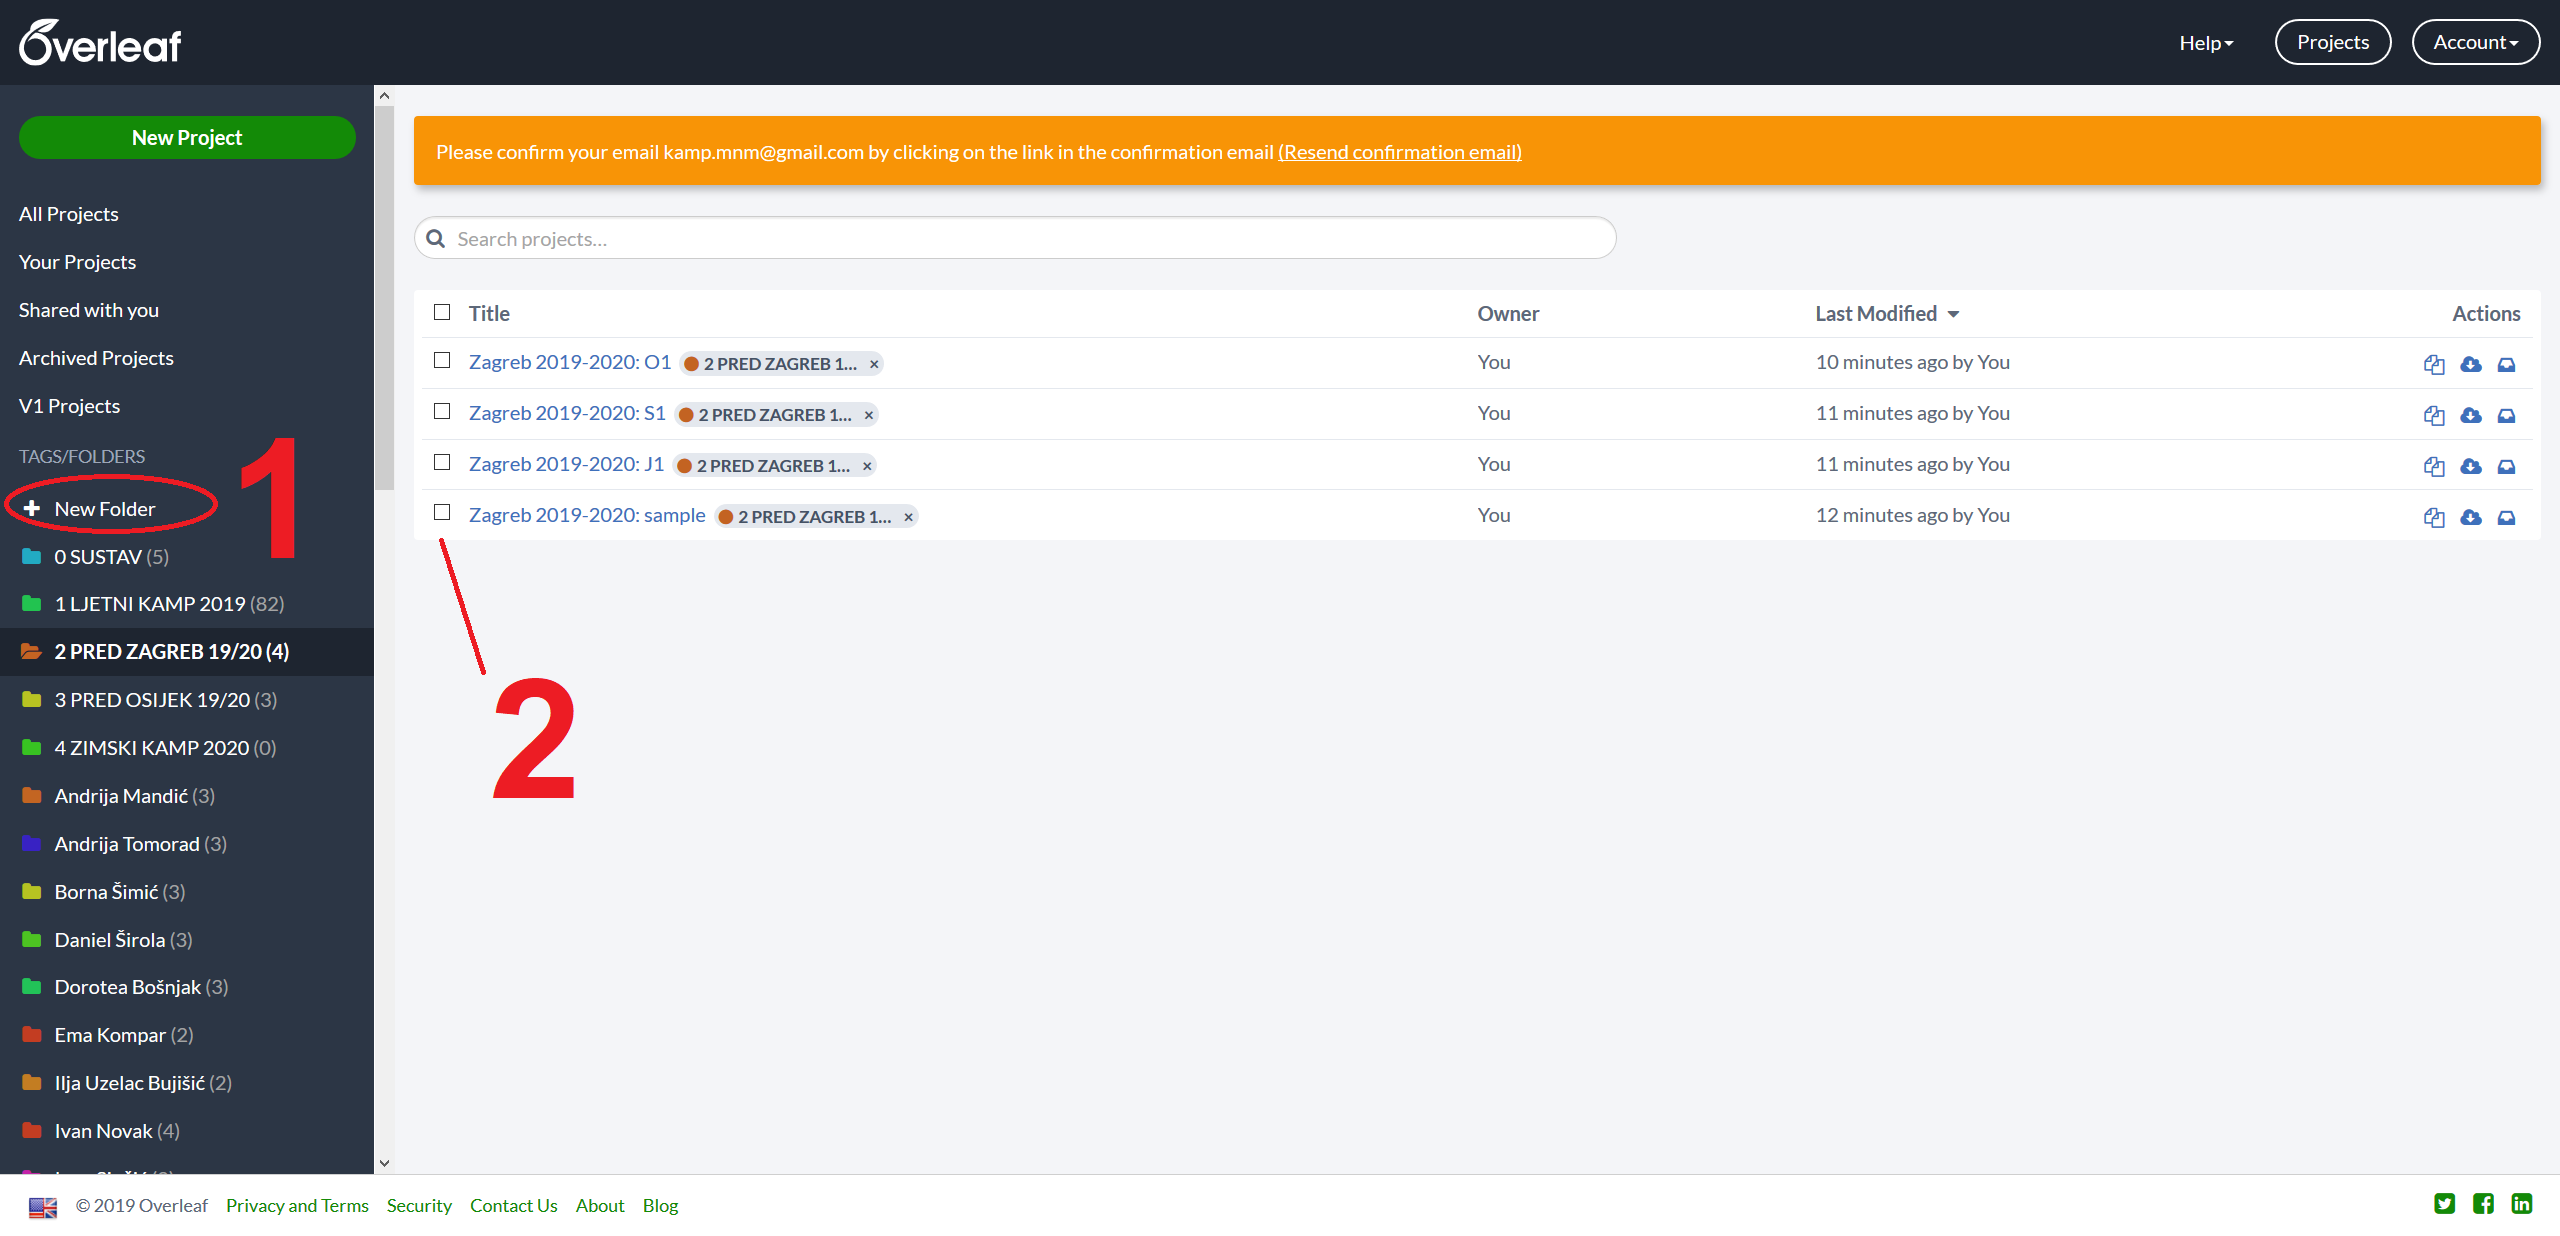
\includegraphics[width = \textwidth]{images/Primjer_1.png}
    \end{figure}
    
    Ukoliko želite
    
    \begin{itemize}
        \item preimenovati postojeće predavanje, pritisnite \textsf{(2a)}, pa \textsf{Rename};
        \item izraditi novo predavanje, pritisnite \textsf{(2a)}, pa \textsf{Make a copy}
        \item premijestiti predavanje u neki folder, pritisnite \textsf{(2b)};
        \item downloadati source, pritisnite \textsf{(2c)};
        \item izbrisati (arhivirati) predavanje, pritisnite \textsf{(2d)}.
    \end{itemize}
    
    \begin{figure}[h]
        \centering
        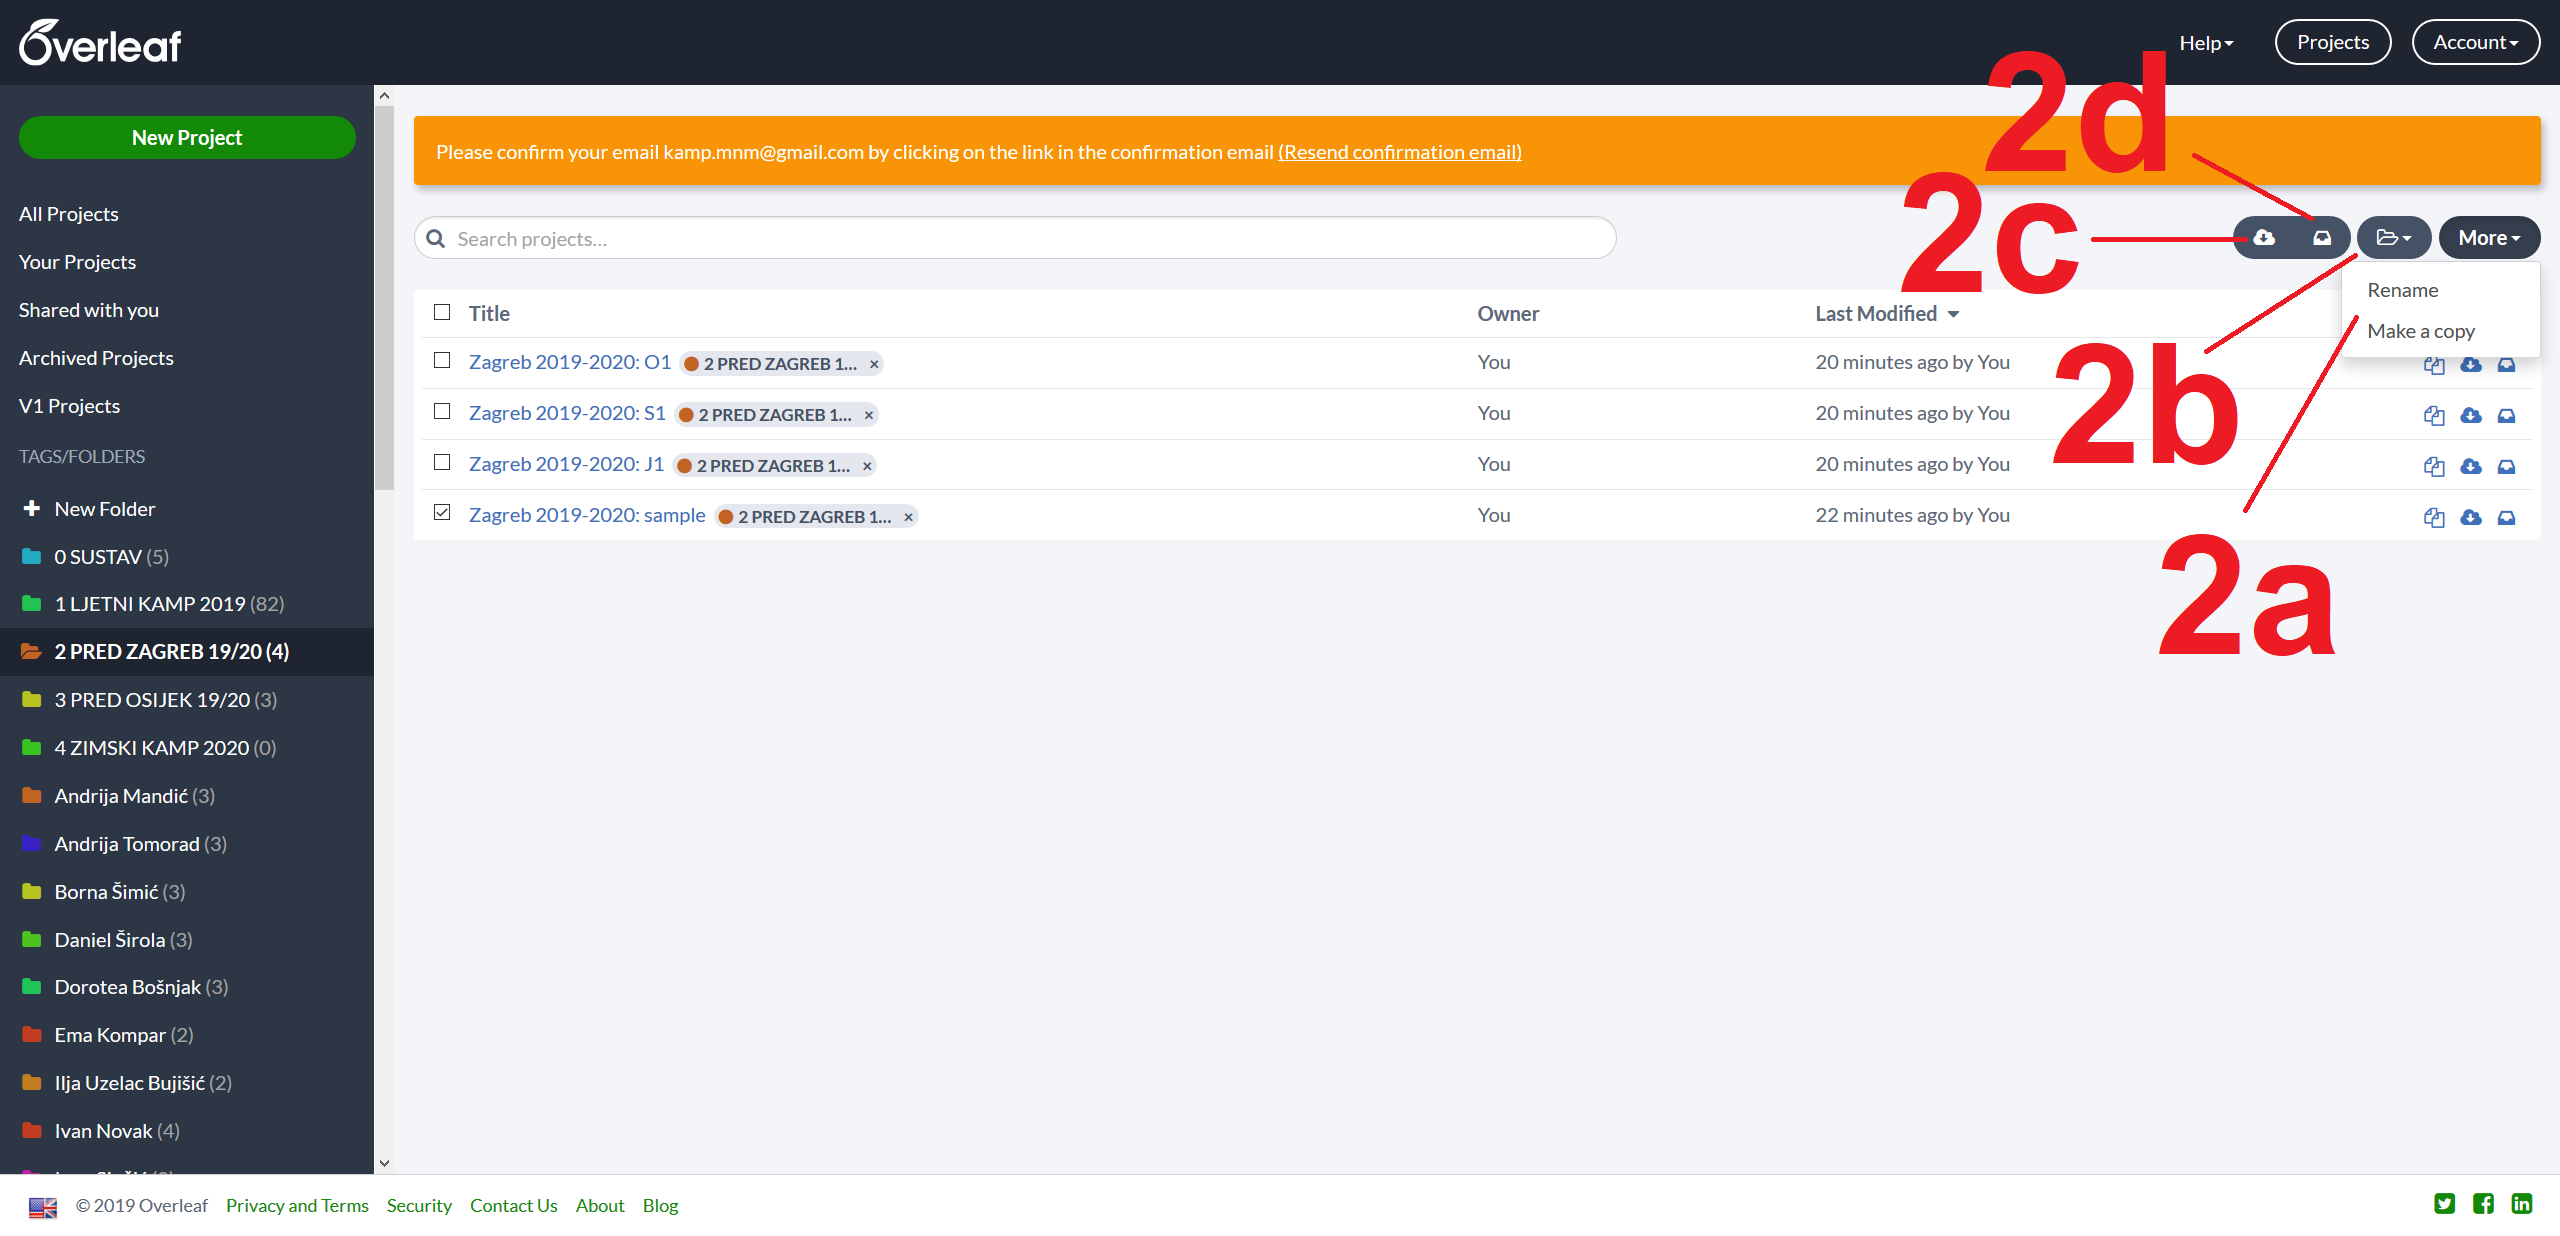
\includegraphics[width = \textwidth]{images/Primjer_2.png}
    \end{figure}
    
\newpage
    
    \section{Unutar filea}
    
    Unutar filea, postoji pet subfilea, redom
    \begin{enumerate}
        \item \textit{1\_naslov.tex} (stavio sam dodatne upute kako što treba promjeniti)
        \item \textit{2\_uvod.tex} (kratki uvod u temu, tamo su opet dodatne upute koja okruženja imate)
        \item \textit{3\_zadaci.tex} (sami zadaci)
        \item \textit{4\_hintovi.tex} (popis hintova za zadatke)
        \item \textit{5\_rjesenja.tex} (popis linkova na zadatke ili ako oni ne postoje onda natipkanja rješenja)
    \end{enumerate}
    
    Potrebno je urediti svih pet, no samo će vam se prva tri ispisati unutar PDF-a (što je regulirano naredbom \textsf{subfile} i možete promjeniti ako želite). Za vidjeti pojedini subfile (npr. \textit{zadaci.tex}), kliknite na njega te izdajte naredbu \textsf{Recompile}, a za vidjeti kako će vam cijelo predavanje izgledati izdajte istu naredbu nakon što je označen \textit{main.tex}. 
    
    \begin{figure}
        \centering
        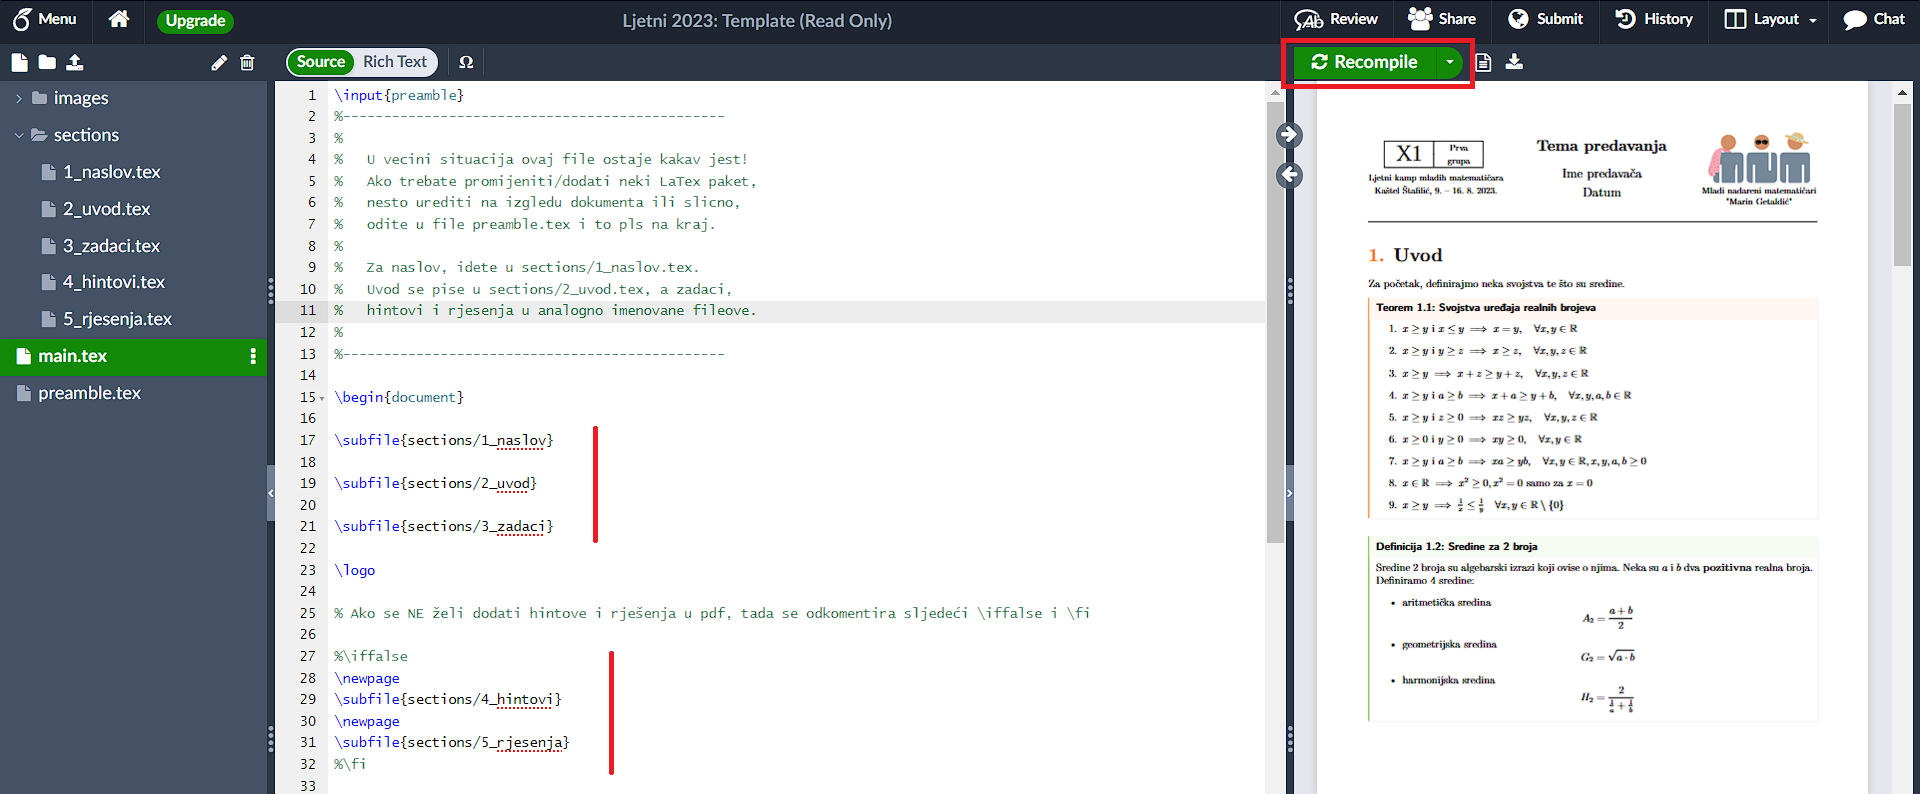
\includegraphics[width = \textwidth]{images/Primjer_3.png}
    \end{figure}
    
    Sve ostalo bi trebalo biti jasnije kroz upute napisane u sourceu, a za ostale dvojbe kojih će sigurno biti, praktički svaki odgovor je dostupan na \url{https://tex.stackexchange.com/} ili da jednostavno postavite pitanje vašoj omiljenoj tražilici, a možete se javiti i meni. :) 
    
    \bigskip
    \printbibliography
\end{document}